\documentclass[a4paper]{article}

%% Language and font encodings
\usepackage[english]{babel}
\usepackage[utf8x]{inputenc}
\usepackage[T1]{fontenc}

%% Sets page size and margins
\usepackage[a4paper,top=3cm,bottom=2cm,left=3cm,right=3cm,marginparwidth=1.75cm]{geometry}

%% Useful packages
\usepackage{amsmath}
\usepackage{graphicx}
\usepackage[colorinlistoftodos]{todonotes}
\usepackage[colorlinks=true, allcolors=blue]{hyperref}
\usepackage[section]{placeins}

\title{Weather Data Analysis Report On Snow Depth}
\author{Zeyu Chen zec003@ucsd.edu}

\begin{document}
\maketitle

\begin{abstract}
The analysis in this report is based on the data from \href{https://www.ncdc.noaa.gov}{NOAA} with a specification of the region from northeast of Nevada to the southwest of Utah (Latitude: (37.0,38.0), Longitude: (-116,-108.0)). The analysis is on the precipitation and snow level based on the PCA analysis and alignment of the latent variables in the PCA.  
\end{abstract}

\section{Data Sanity Check}
The area of our analysis has a precipitation level distributed over two peaks: the first peak happens around around march and the second peak happens around October. The climograph from Cedar city, which is located in the region of the analysis, \href{http://www.usclimatedata.com/climate/cedar-city/utah/united-states/usut0038}{U.S Climate Data} reflects the consistent observation as our data.  The mean of precipitation level does not change much but the standard deviation varies more as the time approaches March and October.
As for the temperature , we can also see that  our data have a consistent observation as the data from  \href{http://www.usclimatedata.com/climate/cedar-city/utah/united-states/usut0038}{U.S Climate Data}. The temperature of the region are high in the summer time and low in the winter time.
\begin{figure}[!htp]
\centering
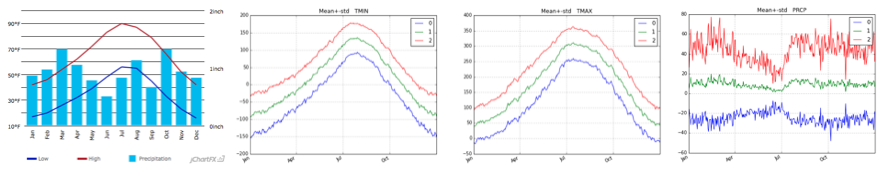
\includegraphics[width=0.95\textwidth]{sanity.png}
\caption{\label{fig:sanity}Form left to right are 1. the climograph from \href{http://www.usclimatedata.com/climate/cedar-city/utah/united-states/usut0038}{U.S Climate Data}. 2. the mean of Min temperature over the year and $\pm$ std. 3. The mean of max temperature over the year and $\pm$ std. 4. The mean precipitation level over the year and $\pm$ the std.}
\end{figure}

\begin{figure}[!htp]
\centering
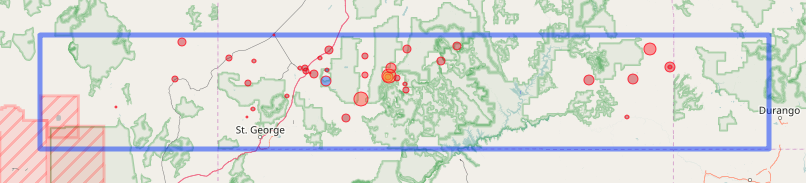
\includegraphics[width=0.95\textwidth]{geo-loc.png}
\caption{\label{fig:geo-loc} The visualization of the geographic locations of those stations. The center of the circle demonstrates the location of the station while the size of the circle demonstrates the amount of data provided by the station.}
\end{figure}

\section{Eigenvector Analysis}
As our data includes different measurements including:
\begin{itemize}
\item TMIN: the minimum temperature of the day.
\item TMAX: the maximum temperature of the day.
\item TOBS: the average temperature for each day. 
\item SNOW: the snow fall level.
\item PRCP: the precipitation level.
\end{itemize}

\noindent However, not all the data are explainable through eigenvectors, so we would like to choose the measurements that are most explainable by our analysis. As showed in the graph below, we can see that some measurements such as TMIN, TOBS, TMAX and SNWD can be well explained through eigenvectors because even just with the top-one eigenvector, we are able to explain around or even more than 40\% of the variance
\begin{figure}[!htp]
\centering
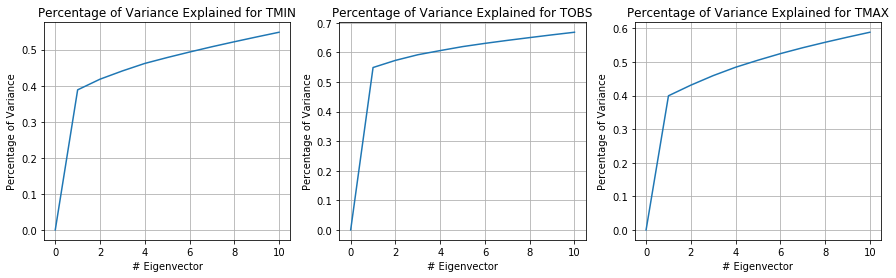
\includegraphics[width=0.95\textwidth]{eigen_1.png}
\caption{\label{fig:t_eigen}Form left to right are the ratio of variance explained by the top-k eigenvectors for TMIN,TOBS and TMAX. We can see that the top-one explains 40\% of variance of TMIN, 55\% of TOBS and 40\% of TMAX. Those measurements can be well explained through eigenvectors}

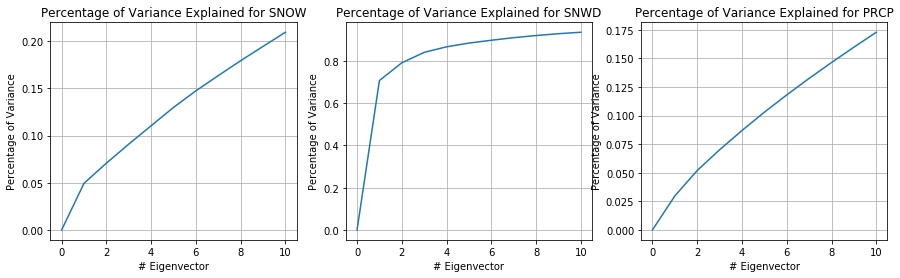
\includegraphics[width=0.95\textwidth]{eigen_2.png}
\caption{\label{fig:t_eigen}Form left to right are the ratio of variance explained by the top-k eigenvectors for SNOW,SNWD and PRCP. We can see that the top-10 eigenvectors only explain 20\% of variance of SNOW, 17.5\% of PRCP while the top one eigenvector explains 70\% of SNWD. Only SNWD can be explained  well through the eigenvectors}

\end{figure}

\section{Snow Depth Analysis}
As discussed above, the eigenvector of snow depth measurement could explain more than 65\% of the variance by the top-one eigenvector alone. It is a good choice to further explore the relation of the eigenvector and the depth of the snow.
\subsection{Eigenvector Interpretation}
As the top-3 eigenvectors can explain more than 80\% percent of the variance of the SNWD measurements, we will be focusing on interpreting those three eigenvectors.

From \ref{fig:eigen_snwd}, we can see that the first eigenvector is negative in both ends of the graph which corresponds to the rising part in the mean graph. The second eigenvector has two peaks while the lowest point is at the high point of the mean graph. The third eigenvector has only one peak at the time of March. 
\noindent From the visualization below \ref{fig:coef1},\ref{fig:coef2},\ref{fig:coef3}, the effect of those eigenvectors can be concluded as below:
\begin{itemize}
\item  eigenvector 1:  the chance of having deep snow depth at spring and the winter of the year v.s. shallow depth of snow at Spring and the Winter of the year.
\item  eigenvector 2: the chance of having deepest snow depth at around February of the year v.s. having deep snow depth at around both March and November of the year.
\item  eigenvector 3: the chance of having relatively deep snow depth at April v.s.  having relatively shallow snow depth At April.
\end{itemize}
\begin{figure}[!htp]
\centering
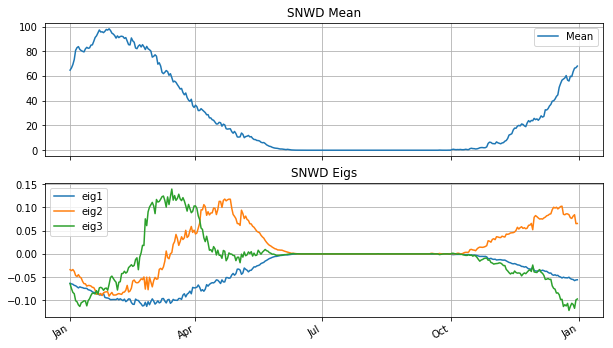
\includegraphics[width=0.95\textwidth]{SNWD.png}
\caption{\label{fig:eigen_snwd} The visualization of the snow depth in terms of mean and top-3 eigenvectors. The top-3 eigenvectors should explain more than 80\% of the variance of the measurement.The meaning of those eigenvectors can be interpret as we change the coefficient of each eigenvector. \ref{fig:coef1},\ref{fig:coef2},\ref{fig:coef3}}
\end{figure}

\begin{figure}[!htp]
\begin{center}
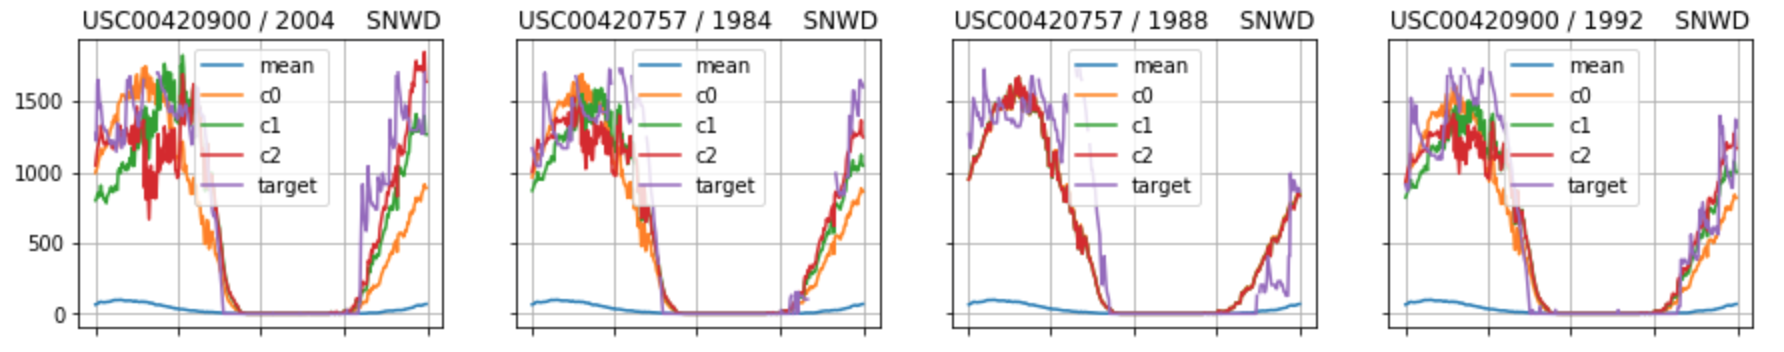
\includegraphics[width=0.95\textwidth]{coef1_neg.png}
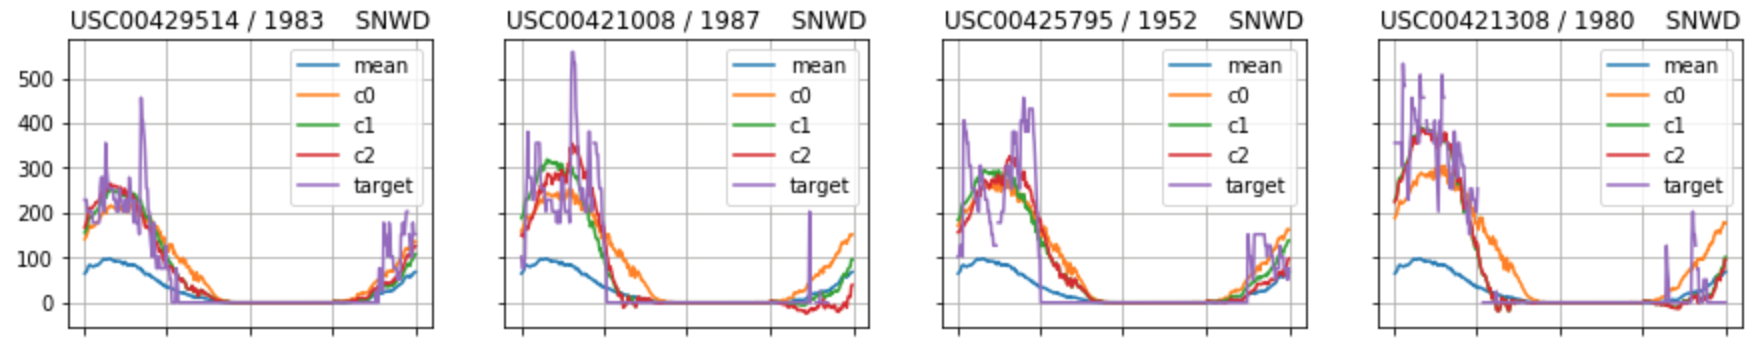
\includegraphics[width=0.95\textwidth]{coef1_pos.png}
\caption{\label{fig:coef1} The visualization of reconstruction of eigenvector 1 with most negative coefficient(first row) and most positive coefficient(second row). With a negative $C0$, the level of snow depth at the spring and winter of the year is much deeper than with a positive $C0$, so we can conclude that eigenvector 1 means the chance of having deep snow depth at spring and the winter of the year v.s. shallow depth of snow at Spring and the Winter of the year.}
\end{center}
\end{figure}

\begin{figure}[!htp]
\vspace{-2cm}
\begin{center}

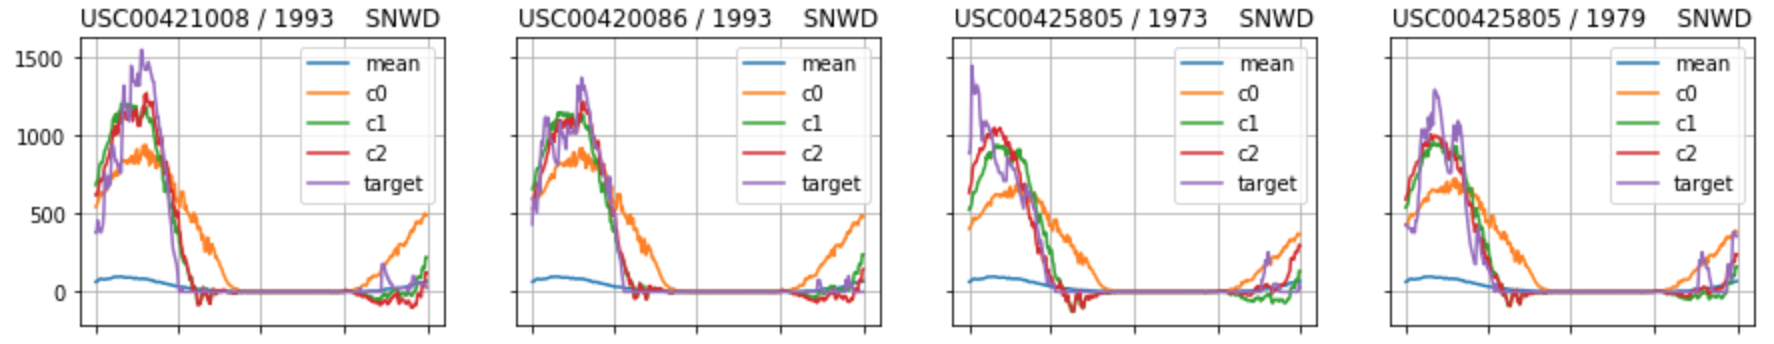
\includegraphics[width=0.95\textwidth]{coef2_neg.png}
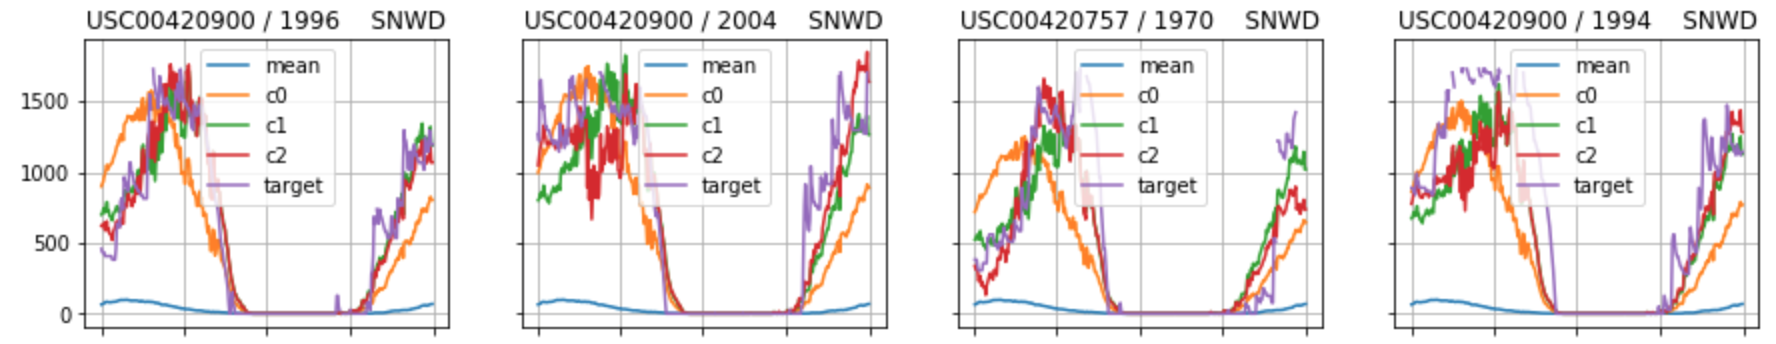
\includegraphics[width=0.95\textwidth]{coef2_pos.png}
\caption{\label{fig:coef2} The visualization of reconstruction of eigenvector 2 with most negative coefficient(first row) and most positive coefficient(second row).With the most negative $C1$, we can see that the peak of the snow depth happens in February of the year with a single spike. If $C1$ is a positive value, we can see two peaks at the time of March and the time of November; therefore we can conclude that the chance of having deepest snow depth at around February of the year v.s. having deep snow depth at around both March and November of the year.}

\vspace{2cm}
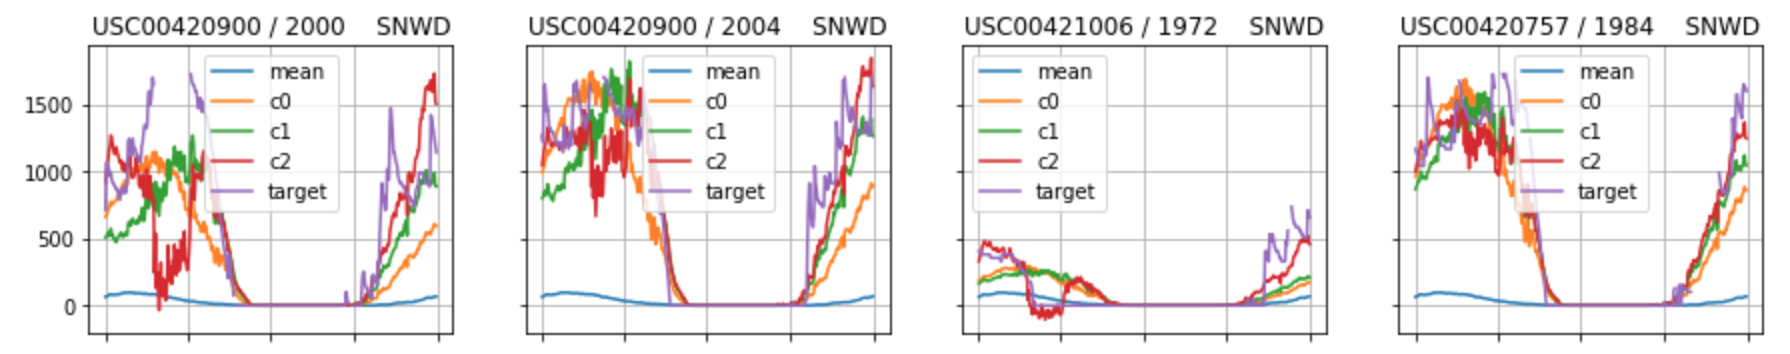
\includegraphics[width=0.95\textwidth]{coef3_neg.png}
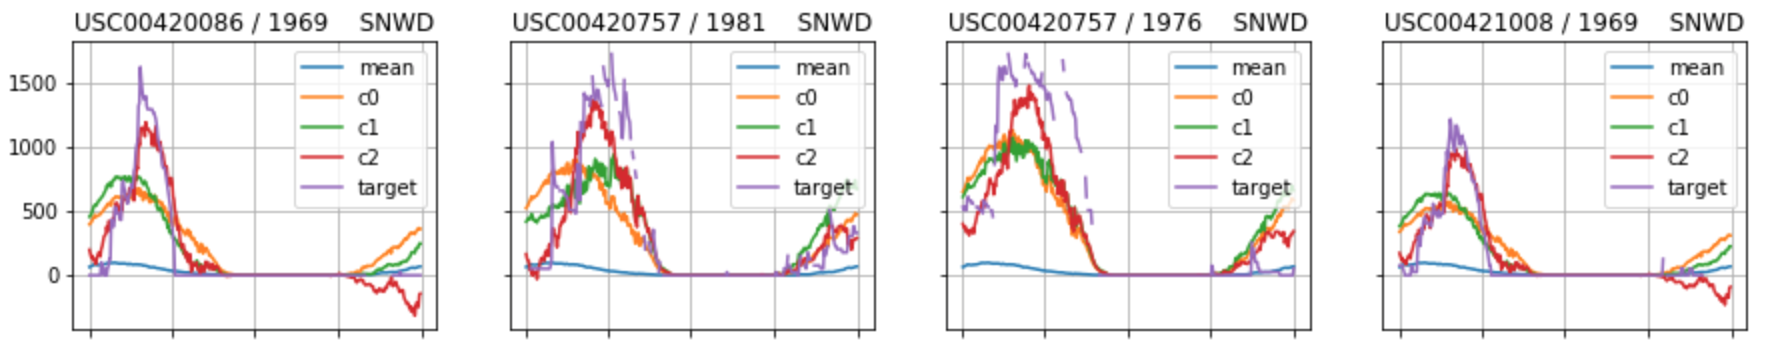
\includegraphics[width=0.95\textwidth]{coef3_pos.png}
\caption{\label{fig:coef3} The visualization of reconstruction of eigenvector 3 with most negative coefficient(first row) and most positive coefficient(second row).With a negative $C2$ value, the depth of snow in April is shallower than the snow depth next to it; however, a very positive $C2$ value corresponds to a peak of snow depth at April; thus we can conclude that eigenvector 3 means the chance of having relatively deep snow depth at April v.s.  having relatively shallow snow depth At April.}

\end{center}
\vspace{-1cm}
\end{figure}

\begin{figure}[!htp]
\centering
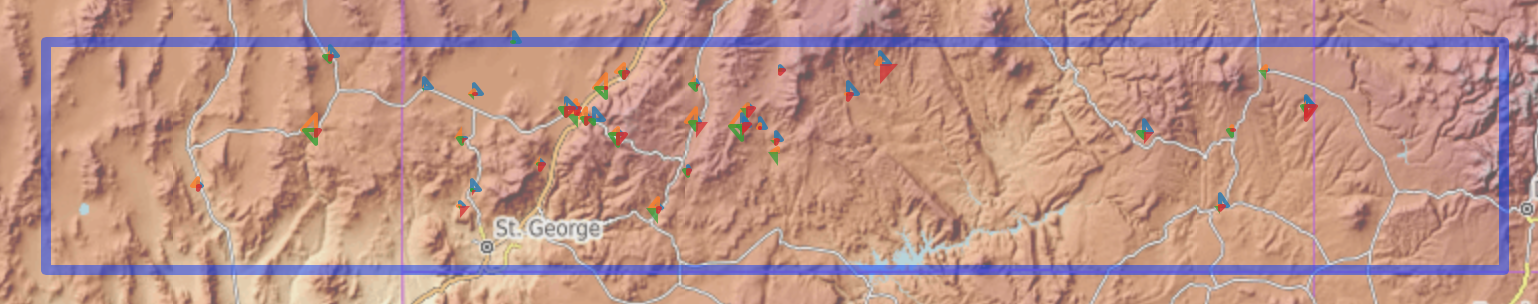
\includegraphics[width=0.8\textwidth]{geo_station.png}
\caption{\label{fig:geo_station} The visualization of the geographic view of stations. Many stations are located in the mountainous areas that are next St. George Utah, but distributed along a wide range of longitude.}
\end{figure}

\subsection{Temporal And Spatial Analysis}
The temporal and spatial effect of the weather system would also be interesting to analyze as most of the stations are located in mountainous areas. In addition, if we pick up four consecutive years of snow depth from one station, we can observe that the snow depth distributed differently in the same station. We can explore whether both temporal and spatial factors will influence the snow depth. As we explained above, the top-3 eigenvectors could explain more than 80\% of the data variance. If we subtract the mean of the data by the year of by station, the variance explained by reconstructing with the eigenvectors can show how important spatial and temporal factors are in our data analysis. As we can see in \ref{tb:mean_spatial}, the spatial and temporal factors both influence the weather system in the area just as we observe from the graphs from our raw data.



\begin{figure}[!htp]
\centering
% 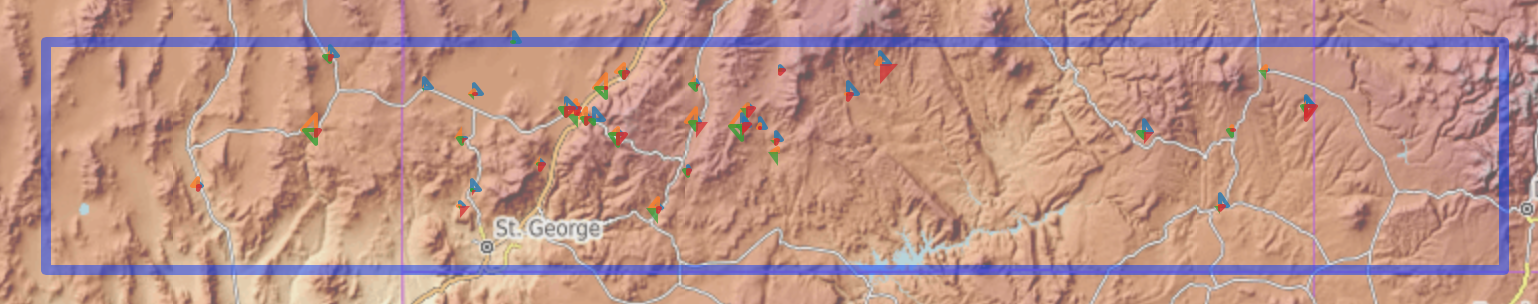
\includegraphics[width=0.8\textwidth]{geo_station.png}
% \caption{\label{fig:geo_station} The visualization of the geographic view of stations. Many stations are located in the mountainous areas that are next St. George Utah, but distributed along a wide range of longitude.}
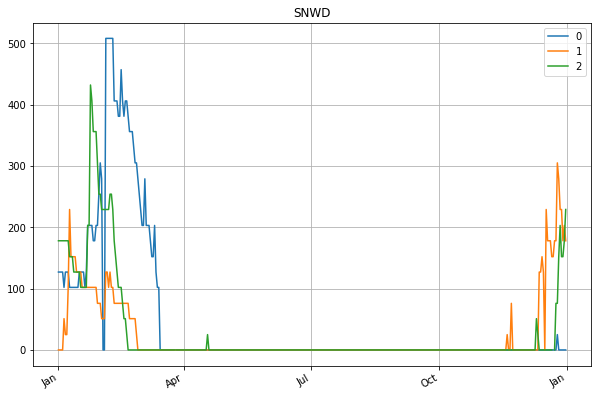
\includegraphics[width=0.95\textwidth]{snow_year.png}
\caption{\label{fig:snow_year} The snow depth data of four consecutive years from station USC00420738. The depth of snow recorded distributed differently year from year.}
\end{figure}

\begin{table}[!htp] \scriptsize \setlength{\tabcolsep}{1pt}
\vspace{-2mm}
\renewcommand{\arraystretch}{1.5}
\begin{center}
\begin{tabular} {c||c||c||c}
%\cline{2-7} 
 MSE Measure &eigenvector 1 + coef\_1&eigenvector 2 + coef\_2&eigenvector 3 + coef\_3\\
 \hline
Original&3018.17985113&1101.73545176&852.415894433\\
 \hline
Remove Mean By Year/(variance explained(\%))&2490.55574671/((17.5\%) &824.529435591/(25.2\%)&661.488079531/(22.4\%)\\
 \hline
Remove Mean By Station/(variance explained(\%)&1436.53471017/(52.4\%)&849.084286192/(22.9\%)&741.409501832/(13.0\%)\\
\hline
\end{tabular}
\caption{\footnotesize we can see that the spatial factor influences the most variance explained using the first eigenvector, while the temporal factor influences more eigenvector 2 and 3 in terms of variance explained.}
\label{tb:mean_spatial}
\end{center}
\end{table}

\section{Conclusion}
From eigenvectors of the data we get, it is reasonable to choose the snow depth to analyze as the top-3 eigenvectors can explain more than 80\% of data variance. By change the eigenvector coefficients, we are able to interpret the meaning of each eigenvector. As we observe the patterns from data, we assume that there should spatial and temporal factors that influence the weather system. With the help of MSE measurement, we are able to quantify the influence and we see that both spatial and temporal factors effects the weather system in the region just as we expect.
\end{document}